\section{OrbitDB}

\begin{figure}[H]
	\centering
	
\includegraphics[width=2cm]{assets/figures/orbitdb-logo.png}
	\caption{OrbitDB logo}
\end{figure}

Η OrbitDB είναι μία P2P βάση δεδομένων ανοιχτού κώδικα. Χρησιμοποιεί το IPFS για την αποθήκευση των δεδομένων και το IPFS Pubsub για τον αυτόματο συγχρονισμό των βάσεων δεδομένων μεταξύ των peers. Είναι μία τελικά συνεπής (eventually consistent) και χρησιμοποιεί CRDTs (Conflict-Free Replicated Data Types) για συγχωνεύσεις βάσεων δεδομένων χωρίς συγκρούσεις, πράγμα που την καθιστά εξαιρετική επιλογή για DApps και offline-first web applications.\cite{2.8-orbitdb}

Κάποια Βασικά χαρακτηριστικά της είναι τα εξής:
\begin{itemize}
	\item \textbf{Stores}: Η OrbitDB παρέχει διάφορους τύπους βάσεων (stores) για διαφορετικά μοντέλα δεδομένων και περιπτώσεις χρήσης:
	
	\begin{itemize}
		\item log: ένα αμετάβλητο (μόνο για προσάρτηση) ημερολόγιο με ανιχνεύσιμο ιστορικό.
		\item feed: ένα μεταβλητό αρχείο καταγραφής με ανιχνεύσιμο ιστορικό, του οποίου οι καταχωρήσεις μπορούν να προστεθούν και να αφαιρεθούν.
		\item keyvalue: μία βάση δεδομένων κλειδιών-τιμών.
		\item docs: μία βάση δεδομένων εγγράφων στην οποία μπορούν να αρχειοθετηθούν έγγραφα JSON με ένα καθορισμένο κλειδί.
		\item counter: μία βάση δεδομένων για καταμέτρηση συμβάντων.
	\end{itemize}
	
	Όλα τα stores υλοποιούνται πάνω στο \texttt{ipfs-log}, μία αμετάβλητη, operation-based CRDT για κατανεμημένα συστήματα, ενώ υπάρχει και η δυνατότητα δημιουργίας προσαρμοσμένων stores ανάλογα με την περίπτωση.
	
	\item \textbf{Address}: Κάθε βάση δεδομένων λαμβάνει κατά τη δημιουργία της μία διεύθυνση της μορφής: \texttt{/orbitdb/CID/DATABASE\_NAME}, όπου CID είναι το IPFS multihash του μανιφέστου της, ενώ το DATABASE\_NAME είναι το όνομα της βάσης\cite{2.8-orbitdb-guide}. Το μανιφέστο είναι ένα IPFS object που περιέχει πληροφορίες της βάσης όπως το όνομα, τον τύπο και έναν δείκτη στον ελεγκτή πρόσβασης (access controller).
	
	\item \textbf{Identity}: Κάθε φορά που προστίθεται μία εγγραφή στη βάση υπογράφεται από τον δημιουργό της, ο οποίος προσδιορίζεται από μία ταυτότητα (identity). Το Identity object, πέρα από τον προεπιλεγμένο τρόπο λειτουργίας, μπορεί να προσαρμοστεί έτσι ώστε να συνδέεται με κάποιο εξωτερικό αναγνωριστικό.
	Η μορφή του έχει ως εξής (βλ. και  \url{https://github.com/orbitdb/orbit-db-identity-provider}):
	
	\begin{figure}[H]
		\centering
		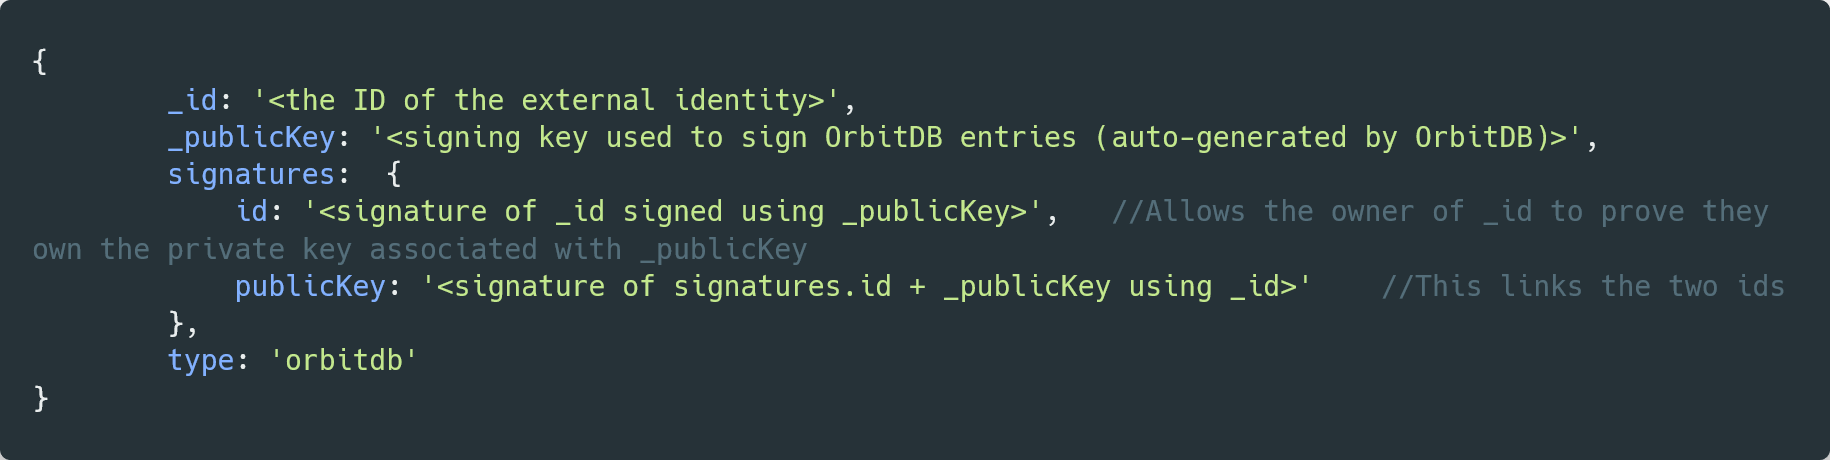
\includegraphics[width=12cm]{assets/figures/orbitdb-identity.png}
		\caption{OrbitDB Identity}
	\end{figure}

	\item \textbf{Access Control}: Κατά τη δημιουργία μίας βάσης μπορούν να οριστούν όσοι θα έχουν δικαίωμα να γράψουν σε αυτήν μέσω ενός ελεγκτή πρόσβασης (access controller). Ο ελεγκτής θα περιλαμβάνει τα public keys τους, τα οποία μπορούν να ανακτηθούν από το identity του καθενός. Από προεπιλογή και αν δεν ορίζεται διαφορετικά, δίνεται πρόσβαση εγγραφής μόνο στον δημιουργό της βάσης.
\end{itemize}
